% Section 3, controlled results (restructure plan, parts 2 and 5). Every number is a macro of
% generated/fresh/numbers.tex (\fv; evidence_ledger_fresh.md names its file and field). Sources:
% results/runs/fresh-v1/{manifest,analysis,analysis_sensitivity}.json and results.jsonl; the verifier specs and the
% contract mappings of tasks/CS-0*; data/controlled/scenarios/CS-0*.json; docs/decision_log.md D61, D62.
\section{Controlled results}
\label{sec:results-controlled}
Under D19, every analysed attempt given the correction is valid (\fv{solve.final}), and \fv{solve.u1} of those given the first request alone are (Table~\ref{tab:fresh-solve}). The \fv{u1.invalid.n} invalid first-request attempts split into \fv{cv.n} correction violators, which break a requirement the correction introduced, and \fv{unspec.n} attempts that only break a base-commit test that the reference passes (the regression norm; CS-02). Table~\ref{tab:fresh-family}, the primary display, gives false acceptance and false rejection per family, and Figure~\ref{fig:fresh-fa} draws them with the correction violators apart from the regression-only attempts; the run's bookkeeping is in the table's caption. Every rate rests on model-proposed labels.

\IfFileExists{generated/fresh/fresh_per_family.tex}{\begin{table}[t]\centering\footnotesize\setlength{\tabcolsep}{4pt}
\caption{Per-family false acceptance and false rejection on the fresh-agent stratum, the primary display (protocol \S15.7), under rule D19's labels: 29 invalid and 50 valid attempts, each distinct graded patch once (79 graded patches; excluded by the reviewed audit: \texttt{CS-02-fresh-A-final-1}). Run \texttt{fresh-v1} graded every pair 3 times under harness 0.3.5 (672 pairs, 0 unresolved). n/a: the family has no attempt of that kind. The second labeler's view: Table~\ref{tab:fresh-family-labeler}. $^{\diamond}$Automated pilot; model-proposed labels, no human labels; 4 controlled families; descriptive (\S\ref{sec:intro}).}\label{tab:fresh-family}
\begin{tabular}{lrrrrrrrrrr}\toprule  & \multicolumn{5}{c}{False acceptance (accepted/invalid)} & \multicolumn{5}{c}{False rejection (rejected/valid)} \\\cmidrule(lr){2-6}\cmidrule(lr){7-11} Condition & CS-01 & CS-02 & CS-03 & CS-04 & Pooled & CS-01 & CS-02 & CS-03 & CS-04 & Pooled \\\midrule
C1 initial-only, plain & 10/10 & 0/2 & 4/7 & 10/10 & 24/29 & 10/10 & 0/17 & 3/13 & 0/10 & 13/50 \\
C2 initial-only, audited & 10/10 & 0/2 & 4/7 & 10/10 & 24/29 & 10/10 & 0/17 & 3/13 & 0/10 & 13/50 \\
C3 correction-aware, plain & 0/10 & 2/2 & 0/7 & 0/10 & 2/29 & 0/10 & 0/17 & 0/13 & 0/10 & 0/50 \\
C4 correction-aware, audited & 0/10 & 2/2 & 0/7 & 0/10 & 2/29 & 0/10 & 0/17 & 6/13 & 0/10 & 6/50 \\
B2 session-LLM baseline & 0/10 & 2/2 & 0/7 & 0/10 & 2/29 & 0/10 & 0/17 & 2/13 & 0/10 & 2/50 \\
B1 repository tests & 0/10 & 0/2 & 0/7 & 0/10 & 0/29 & 8/10 & 17/17 & 9/13 & 0/10 & 34/50 \\
\bottomrule\end{tabular}\end{table}
}{\unfilled{per-family table (make\_tables.py -{}-fresh)}}
\IfFileExists{generated/figures/fresh_fa_fr_by_family.tex}{% Generated by `python paper/make_figures.py`; do not edit. Every value: paper/evidence_ledger_figures.md.
\begin{figure}[t]\centering
\ifdefined\includegraphics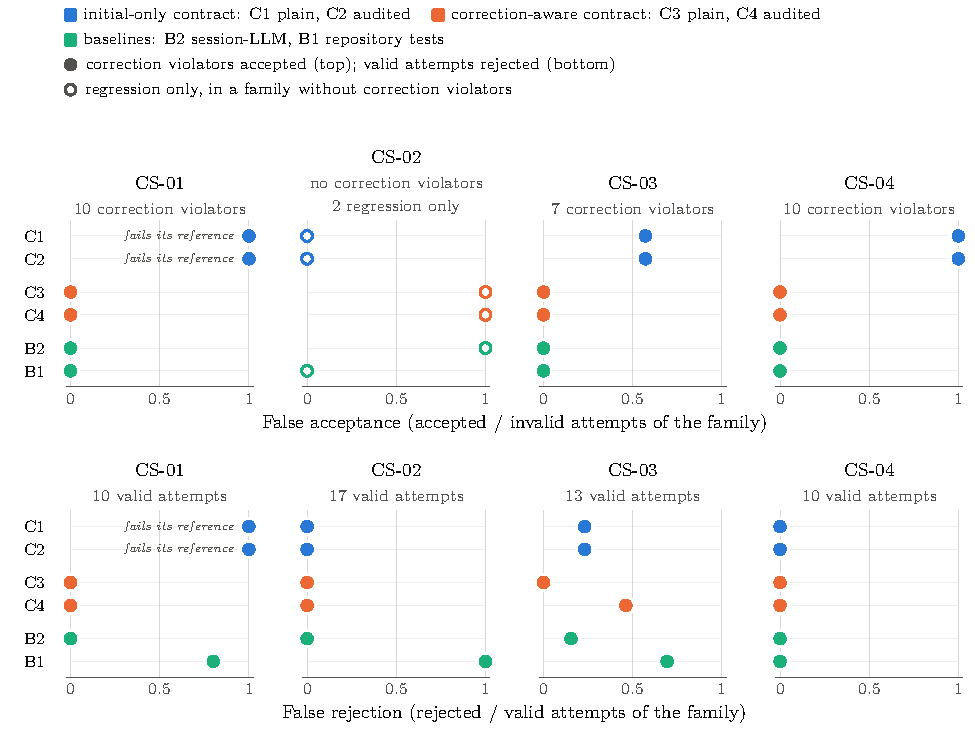
\includegraphics[width=\linewidth]{generated/figures/fresh_fa_fr_by_family.pdf}%
\else\unfilled{figure fresh\_fa\_fr\_by\_family: main.tex must load graphicx}\fi
\caption{False acceptance (top) and false rejection (bottom) per family and condition, run \texttt{fresh-v1}, under rule D19's labels, each distinct graded patch once. Filled marks: correction violators accepted, or valid attempts rejected; hollow marks: a family's invalid attempts when it has no correction violators. Colour: the contract source. Counts: Tables~\ref{tab:fresh-family} and~\ref{tab:fresh-cv}. $^{\diamond}$Automated pilot; model-proposed labels, no human labels; 4 controlled families; descriptive (\S\ref{sec:intro}).}\label{fig:fresh-fa}\label{fig:fresh-fr}
\end{figure}
}{\unfilled{figure fresh\_fa\_fr\_by\_family (make\_figures.py)}}

\subsection{The planned measure, then by behaviour}
\label{sec:results-planned}
The planned measure (protocol~\S15.4, estimand~3) is how C1 and C3 grade the correction violators: C1 accepts \fv{cv.c1} and C3 \fv{cv.c3}. C2 and C4 grade them as C1 and C3 do (\fv{cv.c2}, \fv{cv.c4}), and B2 and B1 accept none (\fv{cv.b2}, \fv{cv.b1}; Table~\ref{tab:fresh-cv}). By behaviour, in a post hoc reading of the secondary reference-gated view (protocol~\S15.7), the families differ as Table~\ref{tab:fresh-behaviours} shows.

\IfFileExists{generated/fresh/fresh_behaviours.tex}{\begin{table}[t]\centering\scriptsize\setlength{\tabcolsep}{2pt}
\caption{What the invalid first-request (\texttt{u1}) attempts of run \texttt{fresh-v1} did, by family, a post hoc reading under rule D19's labels: what the correction changed (the scenario files), which requirements the invalid attempts break (with counts), whether C1 passes the family's reference, how many of C1's checks map to the retracted requirement or to those every violator breaks (both model mappers), how many correction violators C1 and C3 accept (--: the family has none), how many invalid attempts the base-commit tests alone accept, and the invalid attempts whose only violated requirement is the regression norm (Regression only). In CS-01, R-keep-meaningful, introduced in the first request, is broken through the correction's interface: its reference statement and its checks call the correction's keyword \texttt{strip\_trailing\_zero}. $^{\diamond}$Automated pilot; model-proposed labels, no human labels; 4 controlled families; descriptive (\S\ref{sec:intro}).}\label{tab:fresh-behaviours}
\begin{tabular}{l>{\raggedright\arraybackslash}p{0.09\linewidth}>{\raggedright\arraybackslash}p{0.2\linewidth}>{\raggedright\arraybackslash}p{0.11\linewidth}>{\raggedright\arraybackslash}p{0.12\linewidth}>{\raggedright\arraybackslash}p{0.075\linewidth}>{\raggedright\arraybackslash}p{0.075\linewidth}>{\raggedright\arraybackslash}p{0.075\linewidth}>{\raggedright\arraybackslash}p{0.09\linewidth}}\toprule Family & Correction & Invalid \texttt{u1} attempts: what they break & C1 passes its reference & C1 checks on the retracted or broken requirement & C1 accepts & C3 accepts & Base tests accept & Regression only \\\midrule
CS-01 & \raggedright\hspace{0pt}adds 3, retracts 1 & \raggedright\hspace{0pt}10: R-default-unchanged, R-keep-meaningful, R-opt-in, REGRESSION (10); R-custom-format-unchanged (6) & \raggedright\hspace{0pt}no (12 of 14 checks fail) & \raggedright\hspace{0pt}12 of 14 on the retracted R-default-trim & \raggedright\hspace{0pt}10/10 & \raggedright\hspace{0pt}0/10 & \raggedright\hspace{0pt}0/10 & \raggedright\hspace{0pt}0 \tabularnewline
CS-02 & \raggedright\hspace{0pt}adds 4, retracts none & \raggedright\hspace{0pt}2: REGRESSION (2) & \raggedright\hspace{0pt}yes & \raggedright\hspace{0pt}-- & \raggedright\hspace{0pt}-- & \raggedright\hspace{0pt}-- & \raggedright\hspace{0pt}0/2 & \raggedright\hspace{0pt}2 \tabularnewline
CS-03 & \raggedright\hspace{0pt}adds 3, retracts none & \raggedright\hspace{0pt}7: R-all-caps-input (7) & \raggedright\hspace{0pt}yes & \raggedright\hspace{0pt}0 of 14 on R-all-caps-input & \raggedright\hspace{0pt}4/7 & \raggedright\hspace{0pt}0/7 & \raggedright\hspace{0pt}7/7 & \raggedright\hspace{0pt}0 \tabularnewline
CS-04 & \raggedright\hspace{0pt}adds 5, retracts none & \raggedright\hspace{0pt}10: R-zero-step (10) & \raggedright\hspace{0pt}yes & \raggedright\hspace{0pt}0 of 12 on R-zero-step & \raggedright\hspace{0pt}10/10 & \raggedright\hspace{0pt}0/10 & \raggedright\hspace{0pt}10/10 & \raggedright\hspace{0pt}0 \tabularnewline
\bottomrule\end{tabular}\end{table}
}{\unfilled{behaviours table (make\_tables.py -{}-fresh)}}

\paragraph{Silent loss (CS-03, CS-04).} In these families the correction adds \fv{corr.cs03.added.w} and \fv{corr.cs04.added.w} requirements and retracts none, and C1 \fv{ref.c1.cs03} CS-03's reference and \fv{ref.c1.cs04} CS-04's, so a reference gate keeps it. Yet it accepts \fv{cv.silent.c1} of their correction violators (\fv{cv.c1.cs03} in CS-03, \fv{cv.c1.cs04} in CS-04), against \fv{cv.silent.c3} for C3. The violators break \fv{beh.cs03.broken} in CS-03 and \fv{beh.cs04.broken} in CS-04, and no C1 check maps to that requirement (\fv{c1.cs03.checks.broken} of \fv{checks.cs03.c1} checks in CS-03, \fv{c1.cs04.checks.broken} of \fv{checks.cs04.c1} in CS-04; the second model mapper finds \fv{c1.cs03.checks.broken.mapper2} and \fv{c1.cs04.checks.broken.mapper2}). C1 is not asked to test it, and its generator is told not to over-fit the reference diff it is given. The \fv{c1.cs03.cv.rejected} CS-03 violators that C1 rejects fail checks of other requirements of its contract: \fv{c1.cs03.cv.rejected.r4} fail a check of its R4, that \texttt{titleize} behaves as before apart from acronyms, and \fv{c1.cs03.cv.rejected.r3} also a check of its R3, the general acronym rule.

\paragraph{Loud inversion (CS-01).} Here the correction retracts \fv{corr.cs01.superseded.w} requirement of the first request and adds \fv{corr.cs01.added.w} (Figure~\ref{fig:design}c). C1 encodes the retracted request: \fv{c1.cs01.checks.superseded} of its \fv{checks.cs01.c1} checks map to it (\fv{c1.cs01.checks.superseded.mapper2} for the second mapper), and exactly those fail on the reference (\fv{c1.cs01.checks.superseded.failed} of them, and \fv{c1.cs01.checks.other.failed} of the other checks). C1 accepts \fv{cv.c1.cs01} violators and rejects \fv{c1.cs01.fr} valid attempts. A reference gate drops it in CS-01: the gated view loses \fv{og.c1.lost.invalid} invalid and \fv{og.c1.lost.valid} valid attempts, and gated C1 accepts \fv{og.c1.fa} invalid attempts, a denominator that includes CS-02's \fv{unspec.n} regression-only attempts.

\paragraph{No correction violator (CS-02).} None of CS-02's first-request attempts violates the correction (\fv{cv.cs02}). Its \fv{unspec.n} regression-only attempts fail a base test that asserts on a private attribute both removed, pass all \fv{checks.cs02.ref} reference checks, and are valid for the second labeler (D62). C3, C4 and B2 accept them (\fv{unspec.c3}, \fv{unspec.c4}, \fv{unspec.b2}), and they are the whole of those verifiers' false acceptance (\fv{c3.fa}, \fv{c4.fa}, \fv{b2.fa}).

\subsection{The machinery nulls}
\label{sec:results-nulls}
C2 equals C1 on every attempt (difference \fv{cmp.c1-c2.fa.diff} on FA and \fv{cmp.c1-c2.fr.diff} on FR, with no discordant attempt), although its audit failed in CS-01 with the reference not passing, and C2 was frozen as it stood (D27). C4 equals C3 on false acceptance and rejects \fv{c4.fr} valid attempts against C3's \fv{c3.fr}, all in CS-03 (\fv{c4.cs03.fr}). There its audit made \fv{audit.c4.cs03.revisions.w} revision, which added \fv{audit.c4.cs03.added} checks that fix the answers of an audit attack, and of the reference, on edge cases the contracts leave open: contractions, digits and underscores in all-caps words. Of the rejections, \fv{c4.cs03.fr.added} fail only those checks, and the audit record shows no finding after the revision and does not show the added checks (D62). B2 matches C3 and C4 on false acceptance (\fv{b2.fa}); on false rejection it lies between them (\fv{b2.fr}, against \fv{c3.fr} and \fv{c4.fr}). No difference was observed on false acceptance, and \fv{families.w} families cannot show equivalence.

None of the \fv{cmp.count} planned comparisons reaches the unconditional floor of the family-level sign-flip test (\fv{cmp.floor.one} one-sided, \fv{cmp.floor.two} two-sided; Table~\ref{tab:fresh-comparisons}). C1 against C3 on false acceptance (\fv{cmp.c1-c3.fa.diff}) has one-sided $p=\fv{cmp.c1-c3.fa.p.greater}$, above its floor of \fv{cmp.c1-c3.fa.floor}, because CS-02 differs in the other direction (\fv{cmp.c1-c3.fa.cs02}). C1 against C3 and B1 against C4 on false rejection sit at their conditional floors (\fv{cmp.c1-c3.fr.floor} and \fv{cmp.b1-c4.fr.floor}), which the families with no difference set.

\IfFileExists{generated/fresh/fresh_comparisons.tex}{\begin{table}[t]\centering\scriptsize\setlength{\tabcolsep}{4pt}
\caption{The 14 pre-specified paired comparisons on the same units, run \texttt{fresh-v1}, D19 labels. \textbf{All labels are model proposals; no human labels exist.} Metric (n): FA over the invalid or FR over the valid units. A$-$B: pooled difference; then the per-family differences. Disc.: A accepts \& B rejects / A rejects \& B accepts. $p$: exact sign-flip randomization p-values over the 4 families, on the pooled statistic ($>$: A$>$B, $<$: A$<$B, both one-sided; 2-s.: two-sided) and, last but one, two-sided on the family-mean statistic. With 4 families no one-sided $p$ below 0.0625 and no two-sided $p$ below 0.125 can occur; Floor: the smallest one-sided $p$ attainable given the families whose difference is zero. The smallest two-sided $p$ here is 0.25. Short names: C1--C4 contracts (initial or full, plain or audited), B2 full-session LLM, B1 repository tests. Four controlled families: descriptive, not inferential.}\label{tab:fresh-comparisons}
\begin{tabular}{lllrrrrrrrrrrr}\toprule A & B & Metric (n) & A$-$B & CS-01 & CS-02 & CS-03 & CS-04 & Disc. & $p_{>}$ & $p_{<}$ & $p$ 2-s. & $p$ 2-s.\ (mean) & Floor \\\midrule
C1 & C3 & FA (29) & \ensuremath{+}0.76 & \ensuremath{+}1.00 & \ensuremath{-}1.00 & \ensuremath{+}0.57 & \ensuremath{+}1.00 & 24/2 & 0.125 & 0.9375 & 0.25 & 0.625 & 0.0625 \\
C1 & C3 & FR (50) & \ensuremath{+}0.26 & \ensuremath{+}1.00 & 0.00 & \ensuremath{+}0.23 & 0.00 & 0/13 & 0.25 & 1 & 0.5 & 0.5 & 0.25 \\
C2 & C4 & FA (29) & \ensuremath{+}0.76 & \ensuremath{+}1.00 & \ensuremath{-}1.00 & \ensuremath{+}0.57 & \ensuremath{+}1.00 & 24/2 & 0.125 & 0.9375 & 0.25 & 0.625 & 0.0625 \\
C2 & C4 & FR (50) & \ensuremath{+}0.14 & \ensuremath{+}1.00 & 0.00 & \ensuremath{-}0.23 & 0.00 & 5/12 & 0.5 & 0.75 & 1 & 1 & 0.25 \\
C1 & C2 & FA (29) & 0.00 & 0.00 & 0.00 & 0.00 & 0.00 & 0/0 & 1 & 1 & 1 & 1 & 1 \\
C1 & C2 & FR (50) & 0.00 & 0.00 & 0.00 & 0.00 & 0.00 & 0/0 & 1 & 1 & 1 & 1 & 1 \\
C3 & C4 & FA (29) & 0.00 & 0.00 & 0.00 & 0.00 & 0.00 & 0/0 & 1 & 1 & 1 & 1 & 1 \\
C3 & C4 & FR (50) & \ensuremath{-}0.12 & 0.00 & 0.00 & \ensuremath{-}0.46 & 0.00 & 6/0 & 1 & 0.5 & 1 & 1 & 0.5 \\
B2 & C4 & FA (29) & 0.00 & 0.00 & 0.00 & 0.00 & 0.00 & 0/0 & 1 & 1 & 1 & 1 & 1 \\
B2 & C4 & FR (50) & \ensuremath{-}0.08 & 0.00 & 0.00 & \ensuremath{-}0.31 & 0.00 & 4/0 & 1 & 0.5 & 1 & 1 & 0.5 \\
B2 & C3 & FA (29) & 0.00 & 0.00 & 0.00 & 0.00 & 0.00 & 0/0 & 1 & 1 & 1 & 1 & 1 \\
B2 & C3 & FR (50) & \ensuremath{+}0.04 & 0.00 & 0.00 & \ensuremath{+}0.15 & 0.00 & 0/2 & 0.5 & 1 & 1 & 1 & 0.5 \\
B1 & C4 & FA (29) & \ensuremath{-}0.07 & 0.00 & \ensuremath{-}1.00 & 0.00 & 0.00 & 0/2 & 1 & 0.5 & 1 & 1 & 0.5 \\
B1 & C4 & FR (50) & \ensuremath{+}0.56 & \ensuremath{+}0.80 & \ensuremath{+}1.00 & \ensuremath{+}0.23 & 0.00 & 0/28 & 0.125 & 1 & 0.25 & 0.25 & 0.125 \\
\bottomrule\end{tabular}\end{table}
}{\unfilled{comparisons table (make\_tables.py -{}-fresh)}}

\subsection{Repository tests cut both ways}
\label{sec:results-b1}
B1 accepts no invalid attempt (\fv{b1.fa}) and rejects \fv{b1.fr} valid ones. All \fv{b1.fr.added} rejections come from the \fv{b1.checks.added} checks that the session agent added to the reference state's test files; the base commit's \fv{b1.checks.base} checks reject none (\fv{b1.base.fr}; Table~\ref{tab:fresh-b1}). On the base-commit checks alone, B1 would accept \fv{b1.base.fa} invalid attempts (CS-03 \fv{b1.base.fa.cs03}, CS-04 \fv{b1.base.fa.cs04}) and still reject every CS-01 violator (\fv{b1.u1.base.rejected.cs01}). That last part holds partly by construction: the base tests are D19's regression norm, so under D19 they cannot reject a valid attempt, and REGRESSION is among the requirements that every CS-01 violator breaks (\fv{beh.cs01.regression} of \fv{beh.cs01.n}; D62). B1's result concerns agent-written tests carried into the reference, not repository tests in general.

\subsection{Robustness}
\label{sec:results-robust}
The second labeler agrees with D19 on \fv{agree} graded patches ($\kappa=\fv{kappa}$; Table~\ref{tab:fresh-agree}). This is agreement between models of the same model family (configurations B and A), working from the same reference contract, over attempts that cluster into a few behaviours per family. Its \fv{disagree} disagreements are CS-02's regression-only attempts, which it labels valid; under its labels C1 accepts \fv{il.c1.fa} invalid attempts and C3 \fv{il.c3.fa} (Table~\ref{tab:fresh-family-labeler}). Leaving out every flagged attempt (\fv{sens.excluded}; Table~\ref{tab:fresh-sensitivity}), C1 accepts \fv{sens.cv.c1} of the correction violators left and C3 \fv{sens.cv.c3}. The reference-gated view drops C1 in CS-01 only (\fv{og.c1.kept} families kept); there the C1--C3 difference in false acceptance is \fv{og.cmp.c1-c3.fa.diff} over \fv{og.cmp.c1-c3.fa.k} families, with one-sided $p=\fv{og.cmp.c1-c3.fa.p.greater}$ (floor \fv{og.cmp.c1-c3.fa.floor}; Table~\ref{tab:fresh-oracle}). The attempts' solve rates and costs are in Tables~\ref{tab:fresh-solve} and~\ref{tab:fresh-costs}; the cost of generating the verifiers was not recorded (D42).
